% 13-summary.tex
% created 10:41:41 on Thu 14 Mar 2013

%\documentclass[letterpaper,10pt]{article}
\documentclass[twocolumn,10pt,amsmath]{revtex4-1}

\usepackage{graphicx}
\graphicspath{{fig/}}

\usepackage[font=small,format=plain,justification=raggedright]{caption}

%\usepackage[letterpaper]{geometry}

%\usepackage{amsmath}


\begin{document}

\title{Annual report research summary}
\author{Jonah Bernhard}
\date{\today}


\maketitle



\section{Statistical hadronization models}

Heavy-ion collisions produce a hot, dense state of QCD matter commonly known as the quark-gluon plasma (QGP).  The QGP then expands and freezes out into
discrete particles.  If we assume that the QGP is in thermal equilibrium prior to freeze-out, we can use pure statistical mechanics to calculate particle
yields.  Calculated yields may be fit to experimental data to extract thermal parameters of the post-QGP fireball such as temperature and chemical potential.

This approach is generally consistent with experiments at roughly the 10\% level.  However, more precise data have shown that particle production is not purely
statistical.  For example, multiplicities of particles that contain strange quarks do not always match thermal equilibrium values.  Statistical models
accommodate this by including non-equilibrium parameters, which must also be included in fits to data.  For example the strangeness occupancy $\gamma_s$
describes strangeness enhancement:  $\gamma_s = 1$ implies equilibrium, $\gamma_s > 1$ enhancement, $\gamma_s < 1$ suppression.

Currently, there are a number of competing statistical models, and no consensus about the best-fit values of the various parameters, or even which parameters
should be included.  The Duke group plans to help resolve this dispute using SHARE, a flexible statistical model.  Figure \ref{fig:ratiofit} shows a sample
least-squares fit to hadron yield ratios from the STAR experiment at RHIC.  The fit is mostly consistent with data, though the error bars are large.

\begin{figure}[b]
  \centering
  \includegraphics[scale=.7]{star-200}
  \caption{Least-squares fit to identified particle ratios from STAR.}
  \label{fig:ratiofit}
\end{figure}

Standard least-squares fits are susceptible to convergence problems and don't always provide enough information about the quality of the fit.  We apply more
advanced statistical techniques, namely Markov chain Monte Carlo (MCMC), which selects sets of parameters using a Metropolis algorithm and then checks the model's
agreement with data.  This method should provide unbiased information about which parameters are most important and their ideal values.
Figure \ref{fig:mcmc} shows a sample MCMC result from varying temperature and $\gamma_s$ and comparing to the same STAR data as in Fig.\ \ref{fig:ratiofit}.
These preliminary results are consistent with conventional statistical models, as expected.  We anticipate new results this spring.

\begin{figure}[t]
  \centering
  \includegraphics[scale=.7]{mcmc-star-200}
  \caption{MCMC analysis of $T$-$\gamma_s$ dependence using STAR data.  Colors indicate the number of entries in the Markov chain in that bin:  dark red for low
  counts up to yellow for large counts.  The preferred region is in the middle of the ``island'', at $T \sim 165$ MeV and $\gamma_s \sim 1.05$.}
  \label{fig:mcmc}
\end{figure}





\section{Onion visualization}

It is well-known that hadrons with more strange quarks have smaller scattering cross sections, and therefore cease to interact (freeze out) earlier in a post-QGP expansion.  We
seek to visualize the freeze-out surfaces of several baryons with different strangeness:  $\Omega$, $\Xi$, $\Lambda$, and the proton.  The $\Omega$ baryon
consists of three strange quarks ($s=3$), therefore it should interact the least and its freeze-out surface should be smallest.  The $\Xi$ ($s=2$)
should have a somewhat larger surface, followed by the $\Lambda$ ($s=1$) and the proton ($s=0$).  When visualized, these surfaces will take on a layered
appearance, hence the name ``onion visualization''.

Figure \ref{fig:onion} shows freeze-out time distributions sorted by strangeness from pure UrQMD simulations.  It is clear that species with more strangeness
generally freeze out earlier.  Spatial distributions show similar trends.  We expect to have three-dimensional visualizations this spring.

Further work may repeat the analysis with a more realistic model including a hydrodynamic phase.

\begin{figure}[t]
  \centering
  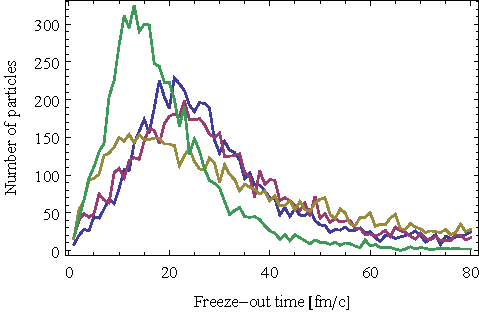
\includegraphics{onion}
  \caption{Freeze-out time distributions for equal numbers of protons (blue), $\Lambda$ (purple), $\Xi$ (tan), and $\Omega$ (green).}
  \label{fig:onion}
\end{figure}





\section{Event-by-event heavy-ion collision simulations}

One of the major goals of heavy-ion physics is to characterize the physical properties of the QGP, perhaps most notably the shear viscosity.  Since it is
impossible to observe the QGP directly, the only way to accomplish this is to compare experimental data to computational models.

%First, the collision must be
%initialized.  The initial state is fed into a relativistic hydrodynamics model, which evolves the QGP until a specified minimum temperature or energy density
%is reached.  Then, hydro is converted to an ensemble of discrete particles.  Finally, a hadronic afterburner, usually UrQMD (Ultra-relativistic Quantum Molecular
%Dynamics) calculates the final scatterings and decays.

A complete simulation of a heavy-ion collision has many components and generally takes at least a few hours on a modern CPU.  Several hours would not be a
problem if the simulation only needed to be carried out once, but every collision is unique, so we cannot realistically model fluctuations with ``average''
events---many complete events must be simulated.  Studies such as this are typically called ``event-by-event''.

We must test many sets of of input parameters in order to determine the best-fit to experiment.  Each set of parameters requires many individual events in order
to acquire adequate statistics.  We expect that several million CPU hours will be required to obtain sufficient data.

In order to satisfy such computational demand, we run the simulations on the Open Science Grid (OSG), which can run hundreds or thousands of events simultaneously on
computers across the USA.

Despite the capabilities of the OSG, we cannot run events at every possible set of input parameters.  We employ a Gaussian statistical emulator to provide
approximate results for points in between explicitly simulated points.  The emulator is similar to a regression or interpolation, but much more powerful:  it supplies
a statistical distribution for every point in parameter space, thus reflecting the true uncertainty of the model.

We will compare simulation data to event-by-event experimental data measured by the ATLAS experiment at the LHC.  ATLAS has measured event-by-event flow
coefficients, which were previously only available integrated over many events.  The flow coefficients---which describe the spatial anisotropy of a given
event---are a sensitive probe of the shear viscosity.   We calculate the flow coefficients from simulated events and compare them
to the corresponding experimental results.
This method enables precise constraints on the shear viscosity and other model
parameters.

The event-by-event model is currently running on the OSG.  We expect to complete the study this summer.




\section{3+1D hydro to micro converter}

Modern heavy-ion collision simulations feature a hydrodynamic phase---which models the physics of the QGP fluid---followed by freeze-out into discrete
particles.  A critical step in any heavy-ion simulation is the conversion from hydrodynamics to an ensemble of particles.

The hydro model evolves until a specified minimum temperature or energy density is reached.  This occurs at many different points in spacetime; all these points
together form a freeze-out hypersurface.  The converter then statistically samples the hypersurface and calculates properties of the emitted particles.  This
is a very computationally intensive process---depending on the model, it may be the longest single step in the full event-by-event simulation.

In our current event-by-event model (see previous section), the hydro component runs in 2+1D (two spatial dimensions and time).  The converter is
designed to read a 2+1D hypersurface and produce a 3+1D particle ensemble.

Eventually, we will replace the 2+1D hydro model with a new 3+1D code, which will also require a new converter.  It must run very efficiently to be viable in an
event-by-event context.

This project is still in preliminary stages.  We expect significant progress this summer and fall.




\end{document}
